\documentclass[12pt,]{book}
\usepackage{lmodern}
\usepackage{setspace}
\setstretch{1.5}
\usepackage{amssymb,amsmath}
\usepackage{ifxetex,ifluatex}
\usepackage{fixltx2e} % provides \textsubscript
\ifnum 0\ifxetex 1\fi\ifluatex 1\fi=0 % if pdftex
  \usepackage[T1]{fontenc}
  \usepackage[utf8]{inputenc}
\else % if luatex or xelatex
  \ifxetex
    \usepackage{mathspec}
  \else
    \usepackage{fontspec}
  \fi
  \defaultfontfeatures{Ligatures=TeX,Scale=MatchLowercase}
\fi
% use upquote if available, for straight quotes in verbatim environments
\IfFileExists{upquote.sty}{\usepackage{upquote}}{}
% use microtype if available
\IfFileExists{microtype.sty}{%
\usepackage{microtype}
\UseMicrotypeSet[protrusion]{basicmath} % disable protrusion for tt fonts
}{}
\usepackage[margin=1in]{geometry}
\usepackage{hyperref}
\hypersetup{unicode=true,
            pdftitle={Building a website using blogdown in R},
            pdfauthor={Alistair Bailey},
            pdfborder={0 0 0},
            breaklinks=true}
\urlstyle{same}  % don't use monospace font for urls
\usepackage{natbib}
\bibliographystyle{apalike}
\usepackage{color}
\usepackage{fancyvrb}
\newcommand{\VerbBar}{|}
\newcommand{\VERB}{\Verb[commandchars=\\\{\}]}
\DefineVerbatimEnvironment{Highlighting}{Verbatim}{commandchars=\\\{\}}
% Add ',fontsize=\small' for more characters per line
\usepackage{framed}
\definecolor{shadecolor}{RGB}{248,248,248}
\newenvironment{Shaded}{\begin{snugshade}}{\end{snugshade}}
\newcommand{\KeywordTok}[1]{\textcolor[rgb]{0.13,0.29,0.53}{\textbf{#1}}}
\newcommand{\DataTypeTok}[1]{\textcolor[rgb]{0.13,0.29,0.53}{#1}}
\newcommand{\DecValTok}[1]{\textcolor[rgb]{0.00,0.00,0.81}{#1}}
\newcommand{\BaseNTok}[1]{\textcolor[rgb]{0.00,0.00,0.81}{#1}}
\newcommand{\FloatTok}[1]{\textcolor[rgb]{0.00,0.00,0.81}{#1}}
\newcommand{\ConstantTok}[1]{\textcolor[rgb]{0.00,0.00,0.00}{#1}}
\newcommand{\CharTok}[1]{\textcolor[rgb]{0.31,0.60,0.02}{#1}}
\newcommand{\SpecialCharTok}[1]{\textcolor[rgb]{0.00,0.00,0.00}{#1}}
\newcommand{\StringTok}[1]{\textcolor[rgb]{0.31,0.60,0.02}{#1}}
\newcommand{\VerbatimStringTok}[1]{\textcolor[rgb]{0.31,0.60,0.02}{#1}}
\newcommand{\SpecialStringTok}[1]{\textcolor[rgb]{0.31,0.60,0.02}{#1}}
\newcommand{\ImportTok}[1]{#1}
\newcommand{\CommentTok}[1]{\textcolor[rgb]{0.56,0.35,0.01}{\textit{#1}}}
\newcommand{\DocumentationTok}[1]{\textcolor[rgb]{0.56,0.35,0.01}{\textbf{\textit{#1}}}}
\newcommand{\AnnotationTok}[1]{\textcolor[rgb]{0.56,0.35,0.01}{\textbf{\textit{#1}}}}
\newcommand{\CommentVarTok}[1]{\textcolor[rgb]{0.56,0.35,0.01}{\textbf{\textit{#1}}}}
\newcommand{\OtherTok}[1]{\textcolor[rgb]{0.56,0.35,0.01}{#1}}
\newcommand{\FunctionTok}[1]{\textcolor[rgb]{0.00,0.00,0.00}{#1}}
\newcommand{\VariableTok}[1]{\textcolor[rgb]{0.00,0.00,0.00}{#1}}
\newcommand{\ControlFlowTok}[1]{\textcolor[rgb]{0.13,0.29,0.53}{\textbf{#1}}}
\newcommand{\OperatorTok}[1]{\textcolor[rgb]{0.81,0.36,0.00}{\textbf{#1}}}
\newcommand{\BuiltInTok}[1]{#1}
\newcommand{\ExtensionTok}[1]{#1}
\newcommand{\PreprocessorTok}[1]{\textcolor[rgb]{0.56,0.35,0.01}{\textit{#1}}}
\newcommand{\AttributeTok}[1]{\textcolor[rgb]{0.77,0.63,0.00}{#1}}
\newcommand{\RegionMarkerTok}[1]{#1}
\newcommand{\InformationTok}[1]{\textcolor[rgb]{0.56,0.35,0.01}{\textbf{\textit{#1}}}}
\newcommand{\WarningTok}[1]{\textcolor[rgb]{0.56,0.35,0.01}{\textbf{\textit{#1}}}}
\newcommand{\AlertTok}[1]{\textcolor[rgb]{0.94,0.16,0.16}{#1}}
\newcommand{\ErrorTok}[1]{\textcolor[rgb]{0.64,0.00,0.00}{\textbf{#1}}}
\newcommand{\NormalTok}[1]{#1}
\usepackage{longtable,booktabs}
\usepackage{graphicx,grffile}
\makeatletter
\def\maxwidth{\ifdim\Gin@nat@width>\linewidth\linewidth\else\Gin@nat@width\fi}
\def\maxheight{\ifdim\Gin@nat@height>\textheight\textheight\else\Gin@nat@height\fi}
\makeatother
% Scale images if necessary, so that they will not overflow the page
% margins by default, and it is still possible to overwrite the defaults
% using explicit options in \includegraphics[width, height, ...]{}
\setkeys{Gin}{width=\maxwidth,height=\maxheight,keepaspectratio}
\IfFileExists{parskip.sty}{%
\usepackage{parskip}
}{% else
\setlength{\parindent}{0pt}
\setlength{\parskip}{6pt plus 2pt minus 1pt}
}
\setlength{\emergencystretch}{3em}  % prevent overfull lines
\providecommand{\tightlist}{%
  \setlength{\itemsep}{0pt}\setlength{\parskip}{0pt}}
\setcounter{secnumdepth}{5}
% Redefines (sub)paragraphs to behave more like sections
\ifx\paragraph\undefined\else
\let\oldparagraph\paragraph
\renewcommand{\paragraph}[1]{\oldparagraph{#1}\mbox{}}
\fi
\ifx\subparagraph\undefined\else
\let\oldsubparagraph\subparagraph
\renewcommand{\subparagraph}[1]{\oldsubparagraph{#1}\mbox{}}
\fi

%%% Use protect on footnotes to avoid problems with footnotes in titles
\let\rmarkdownfootnote\footnote%
\def\footnote{\protect\rmarkdownfootnote}

%%% Change title format to be more compact
\usepackage{titling}

% Create subtitle command for use in maketitle
\newcommand{\subtitle}[1]{
  \posttitle{
    \begin{center}\large#1\end{center}
    }
}

\setlength{\droptitle}{-2em}
  \title{Building a website using blogdown in R}
  \pretitle{\vspace{\droptitle}\centering\huge}
  \posttitle{\par}
  \author{Alistair Bailey}
  \preauthor{\centering\large\emph}
  \postauthor{\par}
  \predate{\centering\large\emph}
  \postdate{\par}
  \date{May 18 2018}


% Preamble
\usepackage[none]{hyphenat}
\usepackage[default,osfigures,scale=0.95]{opensans} % Open sans font
\usepackage[T1]{fontenc} % Use 8-bit encoding that has 256 glyphs
\usepackage{lettrine} % The lettrine is the first enlarged letter at the beginning of the text
\raggedbottom 
\usepackage{makeidx} % These lines add bibliography to TOC
\makeindex
\usepackage[nottoc]{tocbibind}
\renewcommand{\bibname}{References} % Rename biblography as References

\usepackage{amsthm}
\newtheorem{theorem}{Theorem}[chapter]
\newtheorem{lemma}{Lemma}[chapter]
\theoremstyle{definition}
\newtheorem{definition}{Definition}[chapter]
\newtheorem{corollary}{Corollary}[chapter]
\newtheorem{proposition}{Proposition}[chapter]
\theoremstyle{definition}
\newtheorem{example}{Example}[chapter]
\theoremstyle{definition}
\newtheorem{exercise}{Exercise}[chapter]
\theoremstyle{remark}
\newtheorem*{remark}{Remark}
\newtheorem*{solution}{Solution}
\begin{document}
\maketitle

{
\setcounter{tocdepth}{1}
\tableofcontents
}
\listoftables
\listoffigures
\chapter*{Summary}\label{summary}
\addcontentsline{toc}{chapter}{Summary}

These are my instructions for how to build a website using R. The
inspiration came from a series of tweets by
\href{https://twitter.com/dsquintana}{Dan Qunitana} about how to build
an academic website using the
\href{https://bookdown.org/yihui/blogdown/}{blogdown package}
\citep{R-bookdown}.

Following these instructions you can build a website for Bibi the Cat,
using the \href{https://themes.gohugo.io/academic/}{Hugo academic theme}
but you can of course make a website for anything you like and use any
of the many themes available.

These instructions assume you have R \citep{R-base} and
\href{https://www.rstudio.com/}{Rstudio} installed and are reasonably
comfortable using these tools.

For much more detail check out the fantastic
\href{https://bookdown.org/yihui/blogdown/}{blogdown book}.

\chapter{Getting started}\label{getting-started}

\section{Installation}\label{installation}

First you'll need to install the blogdown package:

\begin{Shaded}
\begin{Highlighting}[]
\KeywordTok{install.packages}\NormalTok{(}\StringTok{"blogdown"}\NormalTok{)}
\end{Highlighting}
\end{Shaded}

Then use blogdown to install the static site generator Hugo:

\begin{Shaded}
\begin{Highlighting}[]
\NormalTok{blogdown}\OperatorTok{::}\KeywordTok{install_hugo}\NormalTok{()}
\end{Highlighting}
\end{Shaded}

\section{Installing JabRef}\label{installing-jabref}

If you are going to link academic publications on your website you will
probably find it useful to have \href{http://www.jabref.org/}{JabRef}
installed to create the necessary files you need.

JabRef is an open source bibliography reference manager.

This is not the only way to do things, but it's what I'm familiar with
and is free.

See \protect\hyperlink{creating-publication-files}{the publications
section} for the full details.

\section{Other files}\label{other-files}

If you want to build \href{https://bibi-web.netlify.com/}{Bibi the Cat's
website} you'll need these files.

\chapter{Creating and deploying an initial
website}\label{creating-and-deploying-an-initial-website}

\section{Creating a website in R}\label{creating-a-website-in-r}

We're going to create a website for Bibi the Cat aka The Tiny Tiger.

Here she is:



\begin{figure}

\includegraphics[width=0.5\linewidth]{img/portrait} \caption{Bibi the Cat}\label{fig:bibi-cat}
\end{figure}

Go to
\texttt{File\ \textgreater{}\ New\ Project\ \textgreater{}\ New\ directory}
and then scroll down and choose \textbf{Website using blogdown}.

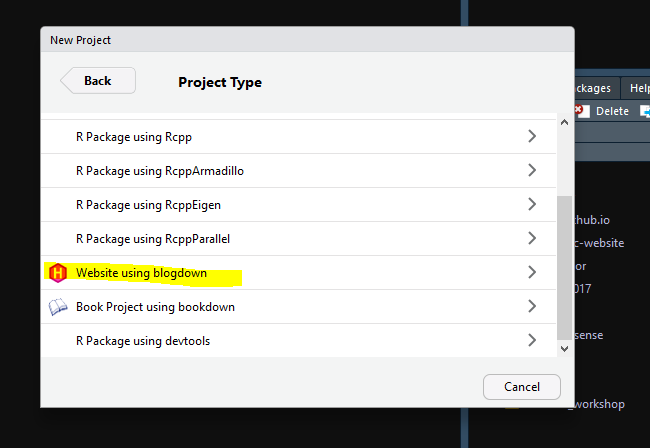
\includegraphics[width=1.2\linewidth]{img/new_website}

This will then take you to the another screen where you can choose the
directory for the website and we choose the theme.

Given Bibi's interests in
\href{https://www.drgoulu.com/wp-content/uploads/2017/09/Rheology-of-cats.pdf}{rheology}
we'll be using the hugo-academic theme, this is selected by entering
\texttt{gchusen/hugo-academic} in the box as shown in Figure
\ref{fig:choose-theme}





\begin{figure}
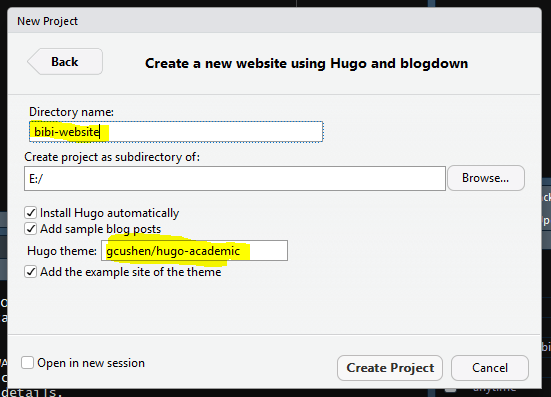
\includegraphics[width=1.2\linewidth]{img/create-website} \caption{Create a new directory with a suitable name with no
spaces and choose a theme, here we're using
\texttt{gchusen/hugo-academic}.}\label{fig:choose-theme}
\end{figure}

Then \texttt{Create\ Project} and it should download the necessary
files, change the working directory to the one created and you should
see something like this:

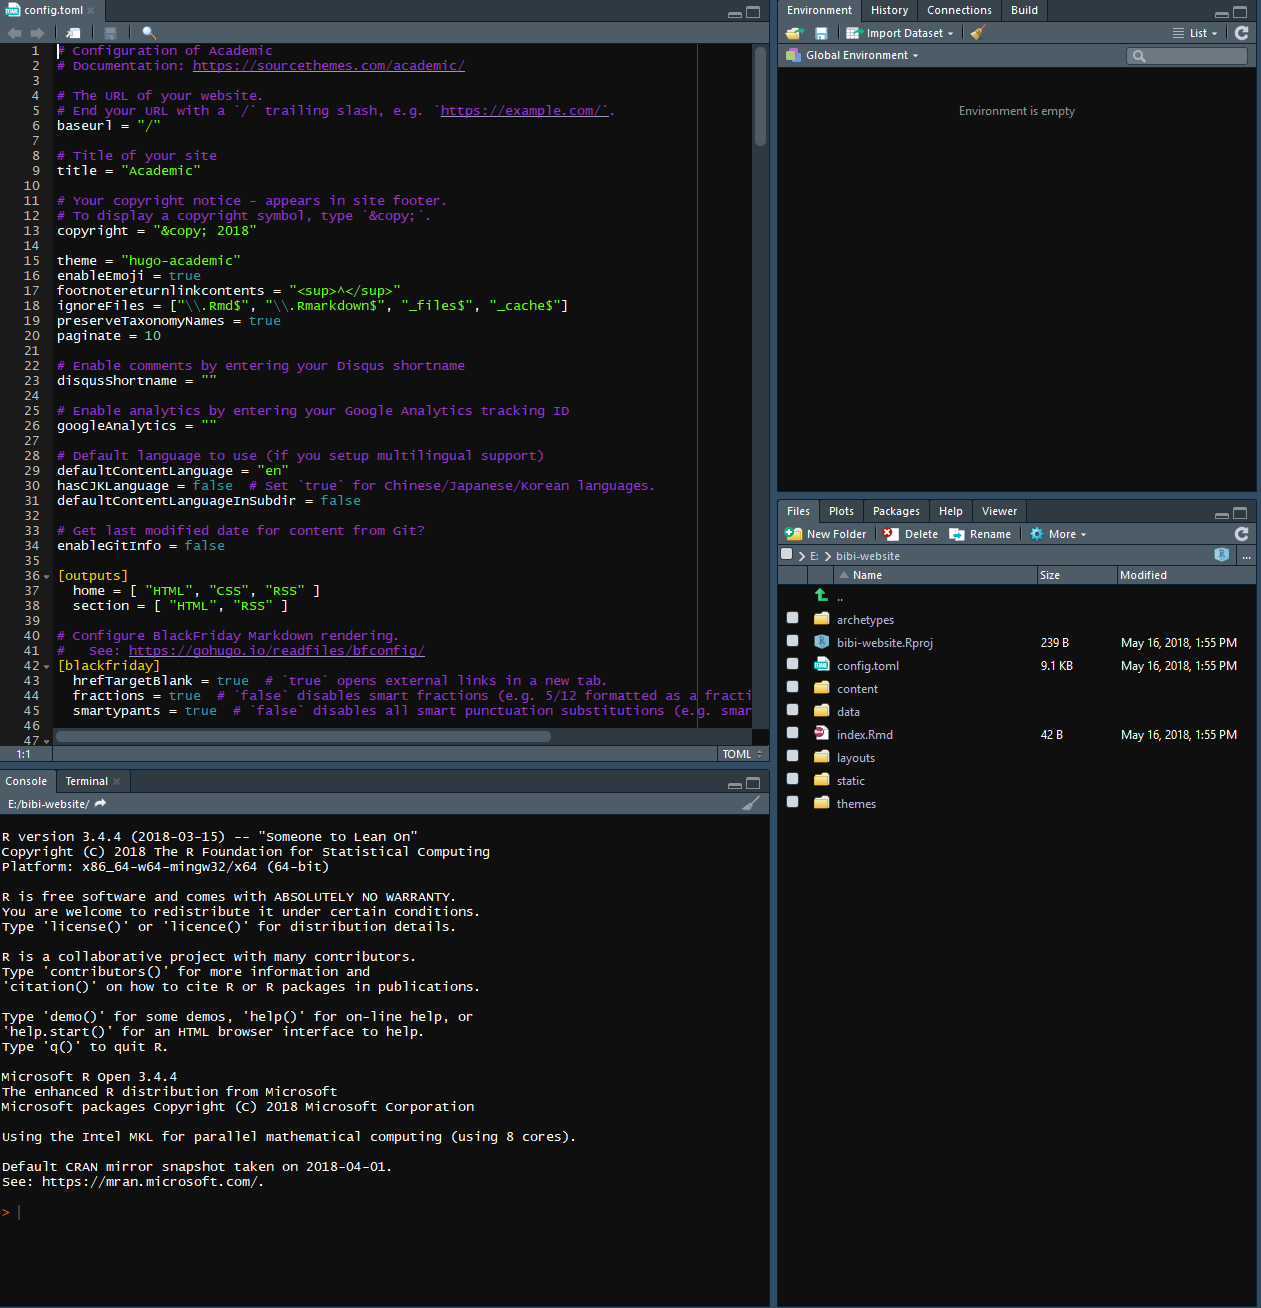
\includegraphics[width=1.2\linewidth]{img/initial-site}

There are a bunch of folders and files, and the script editor pane is
open with the \texttt{confog.toml} file open for editing.

As example files are provided we can build a website immediately using:

\begin{Shaded}
\begin{Highlighting}[]
\NormalTok{blogdown}\OperatorTok{::}\KeywordTok{serve_site}\NormalTok{()}
\end{Highlighting}
\end{Shaded}

And we should see the example site open in the \texttt{Viewer} pane.

\hypertarget{deployment}{\section{Deployment}\label{deployment}}

The simplest way to delpoy our website is to use
\href{https://www.netlify.com/}{netlify}.

Create and account or connect via another account such as
\href{https://github.com/}{GitHub} and then from the \texttt{Sites} tab
that should appear if you click on your name, drag and drop the public
folder from the directory into the box like so:


\includegraphics[width=1.2\linewidth]{img/netlify-drag-public}

Assuming that goes ok, you'll then see a randomly generated name for
your new site. Click on \texttt{Site\ settings} to change the name to
whatever you wish.


\includegraphics[width=1.2\linewidth]{img/netlify-random-sitename}

You should see the option to change the name like so. Click and follow
the instructions.

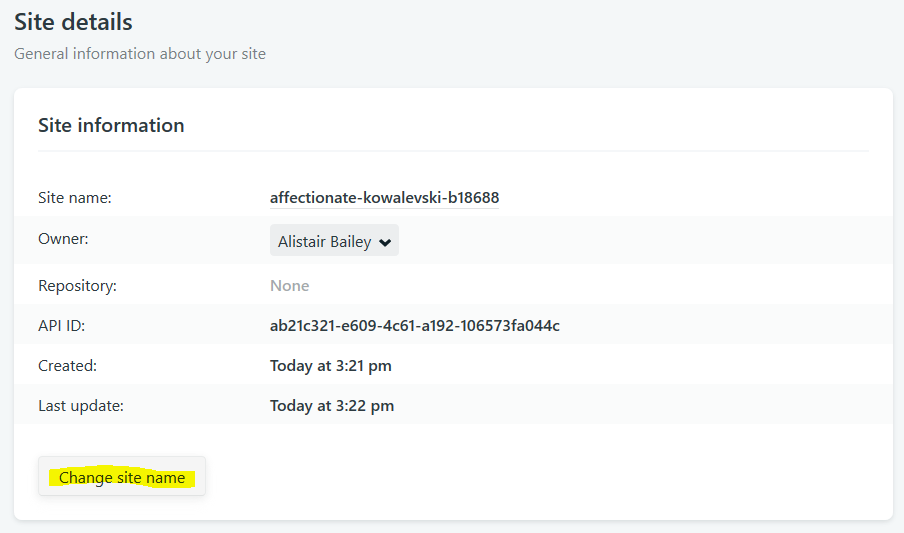
\includegraphics[width=1.2\linewidth]{img/netlify-change-sitename}

Click on your name to get back to \texttt{Sites} and then click on the
name of your website to view it.

Congratulations, you've created and deployed a website.

Next, we'll go back into R to learn how to change the content.

\chapter{Adding content to the site}\label{adding-content-to-the-site}

\section{The file structure in R}\label{the-file-structure-in-r}

The folder containing the published website as we saw in the last
chapter is the \texttt{public} folder.

The \texttt{config.toml} file is where we set the global configurations
for the site.

For detail see the TOML syntax
\href{https://bookdown.org/yihui/blogdown/configuration.html}{blogdown
chapter}, but most of what we're going to change is quite
straightoforward, see \protect\hyperlink{configuration}{Configuration}

The \texttt{content} folder contains subdirectories containing the files
that we create or edit for the sections on the website e.g.~publications
or project pages.

Images and other files we might want (such a CV) go in the
\texttt{static} folder and sub-folders respectively. These will then be
copied to the \texttt{public} folder when we build the site.

We don't need to touch the other folders for the purposes of this
tutorial, but as before the
\href{https://bookdown.org/yihui/blogdown}{blogdown book} has all the
details.

\hypertarget{configuration}{\section{Configuration}\label{configuration}}

Here we'll configure the \texttt{config.toml} file.

\begin{enumerate}
\def\labelenumi{\arabic{enumi}.}
\tightlist
\item
  First we'll change the title:
\end{enumerate}

\begin{Shaded}
\begin{Highlighting}[]
\CommentTok{# Title of your site}
\NormalTok{title =}\StringTok{ "Professor Bibi Cat"}
\end{Highlighting}
\end{Shaded}

\begin{enumerate}
\def\labelenumi{\arabic{enumi}.}
\setcounter{enumi}{1}
\tightlist
\item
  Then we change the details:
\end{enumerate}

\begin{Shaded}
\begin{Highlighting}[]
  \CommentTok{# Your details.}
\NormalTok{  name =}\StringTok{ "Bibi the Cat"}
\NormalTok{  role =}\StringTok{ "Professor of Chaos Theory and Practice"}
  
  \CommentTok{# Organizations/Affiliations.}
  \CommentTok{#   Separate multiple entries with a comma, using the form: }
  \CommentTok{# `[ \{name="Org1", url=""\}, \{name="Org2", url=""\} ]`.}
\NormalTok{  organizations =}\StringTok{ }\NormalTok{[ \{ name =}\StringTok{ "Feline University"}\NormalTok{, url =}\StringTok{ ""}\NormalTok{ \} ]}
\end{Highlighting}
\end{Shaded}

\begin{enumerate}
\def\labelenumi{\arabic{enumi}.}
\setcounter{enumi}{2}
\tightlist
\item
  Next we change the avatar picture by copying an image to
  \texttt{static/img} and either calling it \texttt{potrait.jpg} or
  changing the name in the \texttt{config.toml} file. We'll also change
  the other details, deleting anything we don't want:
\end{enumerate}

\begin{Shaded}
\begin{Highlighting}[]
\NormalTok{  gravatar =}\StringTok{ }\NormalTok{false  }\CommentTok{# Get your avatar from Gravatar.com? (true/false)}
\NormalTok{  avatar =}\StringTok{ "portrait.jpg"}  \CommentTok{# Specify an avatar image (in `static/img/` folder) }
                           \CommentTok{# or delete value to disable avatar.}
\NormalTok{  email =}\StringTok{ "bibi@example.org"}
\NormalTok{  address =}\StringTok{ "Red Fleecy Blanket, Southampton"}
\NormalTok{  office_hours =}\StringTok{ "Whenever I'm hungry"}
\NormalTok{  phone =}\StringTok{ ""}
\NormalTok{  skype =}\StringTok{ ""}
\NormalTok{  telegram =}\StringTok{ ""}
\end{Highlighting}
\end{Shaded}

\begin{enumerate}
\def\labelenumi{\arabic{enumi}.}
\setcounter{enumi}{3}
\tightlist
\item
  Then we'll change the social media icons to include ORCID, this uses
  the \texttt{ai} icon pack, rather than the \texttt{fa} icon pack:
\end{enumerate}

\begin{Shaded}
\begin{Highlighting}[]
\NormalTok{[[params.social]]}
\NormalTok{    icon =}\StringTok{ "orcid"}
\NormalTok{    icon_pack =}\StringTok{ "ai"}
\NormalTok{    link =}\StringTok{ "https://orcid.org/0000-000X-XXXX-XXXX"}

\NormalTok{  [[params.social]]}
\NormalTok{    icon =}\StringTok{ "twitter"}
\NormalTok{    icon_pack =}\StringTok{ "fa"}
\NormalTok{    link =}\StringTok{ "//twitter.com/bibi-the-cat"}
\end{Highlighting}
\end{Shaded}

\begin{enumerate}
\def\labelenumi{\arabic{enumi}.}
\setcounter{enumi}{4}
\tightlist
\item
  We can add, move or remove links that appear on the homepage of the
  website. Bibi is too busy sleeping to write blog posts or do any
  teaching, but she would like to promote her CV which we'll add to the
  \texttt{static/files} folder:
\end{enumerate}

\begin{Shaded}
\begin{Highlighting}[]
\NormalTok{[[menu.main]]}
\NormalTok{  name =}\StringTok{ "Home"}
\NormalTok{  url =}\StringTok{ "#about"}
\NormalTok{  weight =}\StringTok{ }\DecValTok{1}

\NormalTok{[[menu.main]]}
\NormalTok{  name =}\StringTok{ "Publications"}
\NormalTok{  url =}\StringTok{ "#publications"}
\NormalTok{  weight =}\StringTok{ }\DecValTok{2}

\NormalTok{[[menu.main]]}
\NormalTok{  name =}\StringTok{ "CV"}
\NormalTok{  url =}\StringTok{ "/files/cv.pdf"}
\NormalTok{  weight =}\StringTok{ }\DecValTok{3}

\NormalTok{[[menu.main]]}
\NormalTok{  name =}\StringTok{ "Projects"}
\NormalTok{  url =}\StringTok{ "#projects"}
\NormalTok{  weight =}\StringTok{ }\DecValTok{4}


\NormalTok{[[menu.main]]}
\NormalTok{  name =}\StringTok{ "Contact"}
\NormalTok{  url =}\StringTok{ "#contact"}
\NormalTok{  weight =}\StringTok{ }\DecValTok{6}
\end{Highlighting}
\end{Shaded}

Explore to find out what else you can change, such as the publication
format.

\section{Choosing sections and editing the
biography}\label{choosing-sections-and-editing-the-biography}

In the \texttt{content/home} folder are a series of files which
configure the sections widgets.

To turn a section off, open the relevant file and change
\texttt{active\ =\ true} to \texttt{active\ =\ false}.

For example, Bibi is far too busy sleeping to do any teaching, so we'll
turn of the teaching widget by opening \texttt{teaching.md} and changing
the \texttt{active} status.

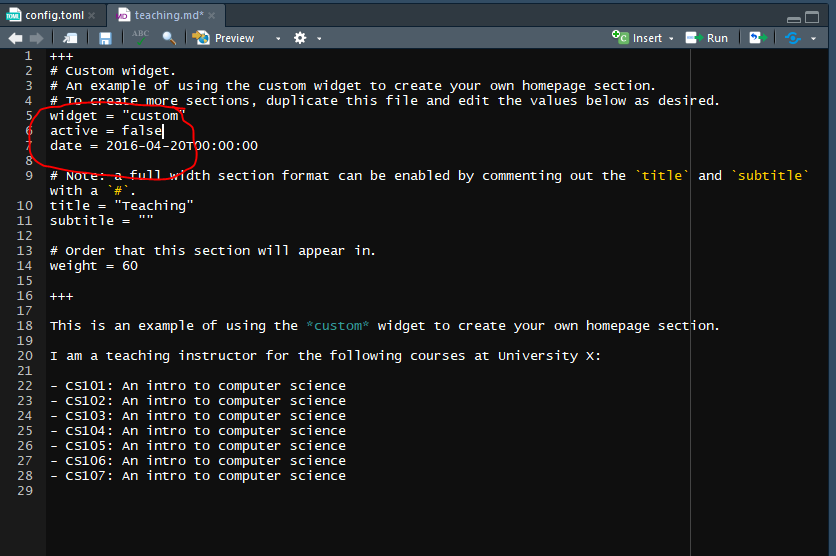
\includegraphics[width=1.2\linewidth]{img/turn-off-widget}

Let's do this for \texttt{hero}, \texttt{publications\_selected},
\texttt{posts},\texttt{talks} and \texttt{teaching}.

And now look at the updated site. \texttt{hero} controlled the top
banner, and \texttt{publications} is where the link on our menu bar
links to.

\section{Editing section content}\label{editing-section-content}

The template files in \texttt{content/home} are written in markdown,
lightweight markup language, where for example \texttt{\#} indicates
Heading 1 and \texttt{\#\#} Heading 2. See the
\href{https://github.com/adam-p/markdown-here/wiki/Markdown-Cheatsheet}{markdown
cheatsheet} to quickly understand the syntax.

You can also write Rmarkdown files here, we're not going to, but see
\href{https://bookdown.org/yihui/blogdown/output-format.html}{here} for
details.

Starting with the \texttt{about} file, the bit between the \texttt{+++}
symbols is for the \texttt{about} widget that creates the interests and
education bit on the homepage.

\begin{Shaded}
\begin{Highlighting}[]
\OperatorTok{+++}
\CommentTok{# About/Biography widget.}
\NormalTok{widget =}\StringTok{ "about"}
\NormalTok{active =}\StringTok{ }\NormalTok{true}
\NormalTok{date =}\StringTok{ }\DecValTok{2016}\OperatorTok{-}\DecValTok{04}\OperatorTok{-}\NormalTok{20T00}\OperatorTok{:}\DecValTok{00}\OperatorTok{:}\DecValTok{00}

\CommentTok{# Order that this section will appear in.}
\NormalTok{weight =}\StringTok{ }\DecValTok{5}

\CommentTok{# List your academic interests.}
\NormalTok{[interests]}
\NormalTok{  interests =}\StringTok{ }\NormalTok{[}
    \StringTok{"Sleeping"}\NormalTok{,}
    \StringTok{"Cardboard boxes and bags"}\NormalTok{,}
    \StringTok{"Dreamies"}
\NormalTok{  ]}

\CommentTok{# List your qualifications (such as academic degrees).}
\NormalTok{[[education.courses]]}
\NormalTok{  course =}\StringTok{ "PhD in Causing Chaos"}
\NormalTok{  institution =}\StringTok{ "University of Life"}
\NormalTok{  year =}\StringTok{ }\DecValTok{2012}

\NormalTok{[[education.courses]]}
\NormalTok{  course =}\StringTok{ "MEng in Cardboard Box Destruction"}
\NormalTok{  institution =}\StringTok{ "University of Life"}
\NormalTok{  year =}\StringTok{ }\DecValTok{2009}

\NormalTok{[[education.courses]]}
\NormalTok{  course =}\StringTok{ "BSc in Covering Everything in Hair"}
\NormalTok{  institution =}\StringTok{ "University of Life"}
\NormalTok{  year =}\StringTok{ }\DecValTok{2008}
 
\OperatorTok{+++}

\CommentTok{# Biography}

\NormalTok{Bibi the Cat is a Professor }\ControlFlowTok{in}\NormalTok{ Chaos Theory and Practice. }\DecValTok{90}\NormalTok{% of her time is}
\NormalTok{spent snoozing, whilst she devotes the other }\DecValTok{10}\NormalTok{% to destroying things and }
\NormalTok{eating tasty treats. Don}\StringTok{'t call her, she'}\NormalTok{ll call you.}
\end{Highlighting}
\end{Shaded}

\section{Creating Projects content}\label{creating-projects-content}

Now if we go up to the \texttt{content} directory you'll see we have
folders for \texttt{projects} and \texttt{publication}.

Let's go into \texttt{content/project} and open
\texttt{deep-learning.md} and edit it, starting with the widget section
to change:

\begin{enumerate}
\def\labelenumi{\arabic{enumi}.}
\tightlist
\item
  the date
\item
  the title
\item
  the summary
\item
  the preview image to the one in \texttt{static/img}
\item
  the tags
\item
  the header image also to ehe one in \texttt{static/img}
\end{enumerate}

And then write whatever we want to about the project, below the
\texttt{+++} , I've added some markdown for another image also in the
\texttt{static/img/} folder so we have this:

\begin{Shaded}
\begin{Highlighting}[]
 \OperatorTok{+++}
\CommentTok{# Date this page was created.}
\NormalTok{date =}\StringTok{ }\DecValTok{2018}\OperatorTok{-}\DecValTok{05}\OperatorTok{-}\NormalTok{17T00}\OperatorTok{:}\DecValTok{00}\OperatorTok{:}\DecValTok{00}

\CommentTok{# Project title.}
\NormalTok{title =}\StringTok{ "Bags"}

\CommentTok{# Project summary to display on homepage.}
\NormalTok{summary =}\StringTok{ "Bibi loves to get into bags"}

\CommentTok{# Optional image to display on homepage (relative to `static/img/` folder).}
\NormalTok{image_preview =}\StringTok{ "bibi-bag.jpg"}

\CommentTok{# Tags: can be used for filtering projects.}
\CommentTok{# Example: `tags = ["machine-learning", "deep-learning"]`}
\NormalTok{tags =}\StringTok{ }\NormalTok{[}\StringTok{"bags"}\NormalTok{]}

\CommentTok{# Optional external URL for project (replaces project detail page).}
\NormalTok{external_link =}\StringTok{ ""}

\CommentTok{# Does the project detail page use math formatting?}
\NormalTok{math =}\StringTok{ }\NormalTok{false}

\CommentTok{# Optional featured image (relative to `static/img/` folder).}
\NormalTok{[header]}
\NormalTok{image =}\StringTok{ "bibi-bag.jpg"}
\NormalTok{caption =}\StringTok{ "Bibi in a bag"}

\OperatorTok{+++}

\NormalTok{I love bags, but also boxes. In fact anything I can get inside, especially}
\ControlFlowTok{if}\NormalTok{ you don}\StringTok{'t want me to.}

\StringTok{![Bibi in a box](/img/bibi-box.jpg)}
\end{Highlighting}
\end{Shaded}

I then save this as \texttt{bags.md} and delete the
\texttt{deep-learning.md} file.

I'll leave you to explore the external link example, but it requires
editing the widget as before for title, date and images, and then
changing the link to your external webpage.

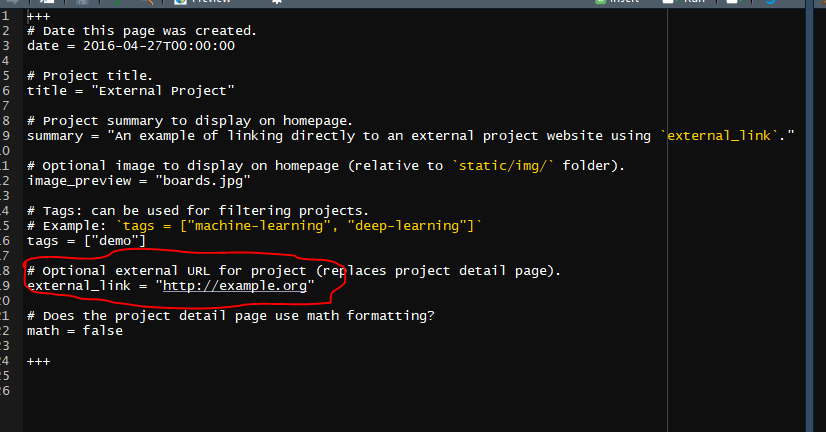
\includegraphics[width=1.2\linewidth]{img/external-link-project}

In the next chapter we'll look at adding publications to the site.

\section{Troubleshooting}\label{troubleshooting}

When you start changing things, you may find that the site stops
automatically updating. This indicates an error.

To find out what is wrong, go to the \texttt{Terminal} tab in Rstudio
and type \texttt{hugo\ -v} and try to figure it out.

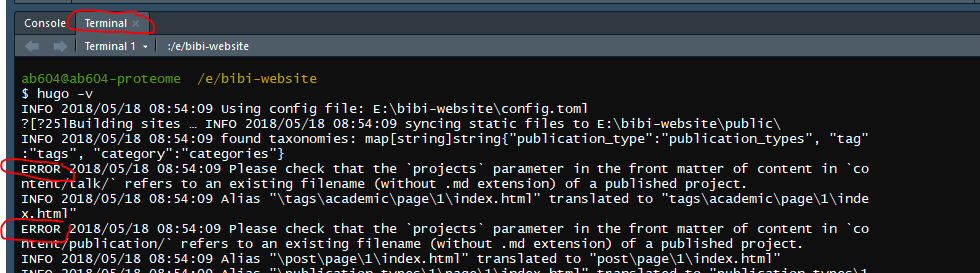
\includegraphics[width=1.2\linewidth]{img/hugo-error}

Here, I've removed \texttt{deep-learning.md} from the project folder,
but the error indicated there are references to it in other files that I
needed to amend.

For the first error, I opened the \texttt{content/talk/} folder and in
the \texttt{example-talk.md} file I see that line 19 has
\texttt{projects\ =\ {[}"deep-learnig"{]}} . So I commented it out with
a \texttt{\#} symbol.

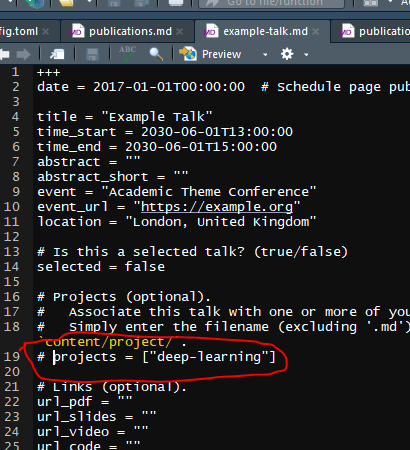
\includegraphics[width=1.2\linewidth]{img/hugo-error2}

Follow the same approach for all errors until when you run
\texttt{hugo\ -v} there are no more, and the site should now build.

\hypertarget{creating-publication-files}{\chapter{Creating publication
files}\label{creating-publication-files}}

This is probably the most fiddly part. In the
\texttt{content/publication} folder we need \texttt{.md} files for each
publication we want to add to our site.

Bibi being quite a lazy cat only has one publication, but we'll look at
how to automate the process for many.

\section{Citation format}\label{citation-format}

To add publication citations, we first need them in \texttt{bibtex}
format. This can be done using \href{http://www.jabref.org/}{JabRef}.

\begin{enumerate}
\def\labelenumi{\arabic{enumi}.}
\tightlist
\item
  Open JabRef and go to
  \texttt{Options\ \textgreater{}\ Preferences\ \textgreater{}\ General}
  and ensure \texttt{Default\ encoding} is set to \texttt{UTF-8}
\end{enumerate}

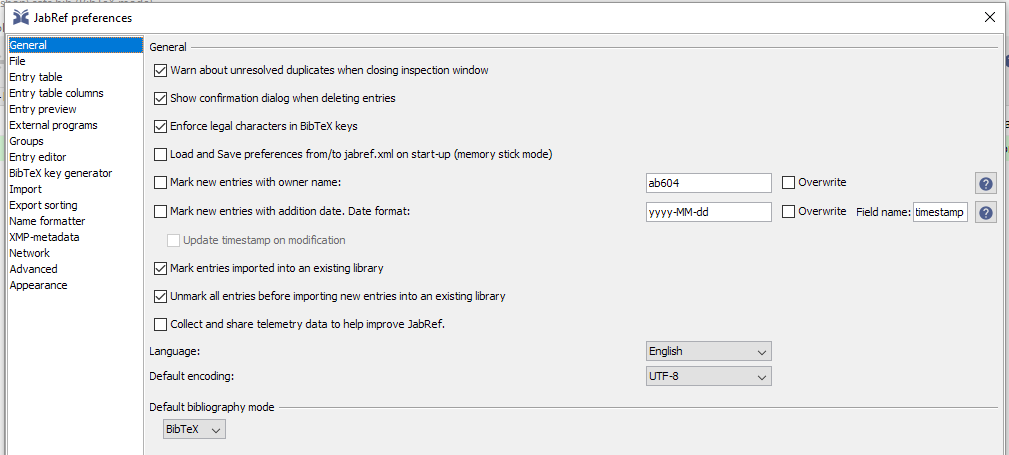
\includegraphics[width=1.2\linewidth]{img/jabref_general_settings}

\begin{enumerate}
\def\labelenumi{\arabic{enumi}.}
\setcounter{enumi}{1}
\tightlist
\item
  Then go to
  \texttt{Options\ \textgreater{}\ Preferences\ \textgreater{}\ Bibtex\ key\ generator}
  and set this to \texttt{{[}auth:lower{]}{[}year{]}} and then
  \texttt{OK}.
\end{enumerate}

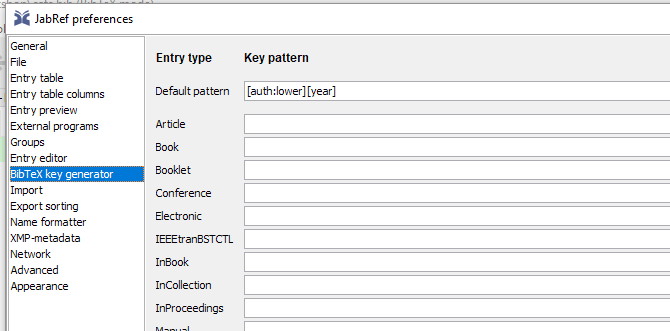
\includegraphics[width=1.2\linewidth]{img/jabref_bibtex_key}

\begin{enumerate}
\def\labelenumi{\arabic{enumi}.}
\setcounter{enumi}{2}
\item
  Then create a library
  \texttt{File\ \textgreater{}\ New\ Bibtex\ Library}.
\item
  If you have exported your publications from EndNote or other software
  as bibtex you can import this into your new library and then highlight
  the list and click on the key icon to generate bibtex keys.
\item
  Alternatively, we can generate the list using the search function,
  here I entered a DOI and searched with Google Scholar:
\end{enumerate}

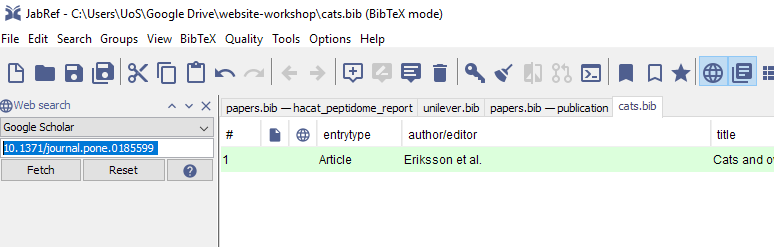
\includegraphics[width=1.2\linewidth]{img/jabref_websearch}

Then I selected the publication and generated the key.

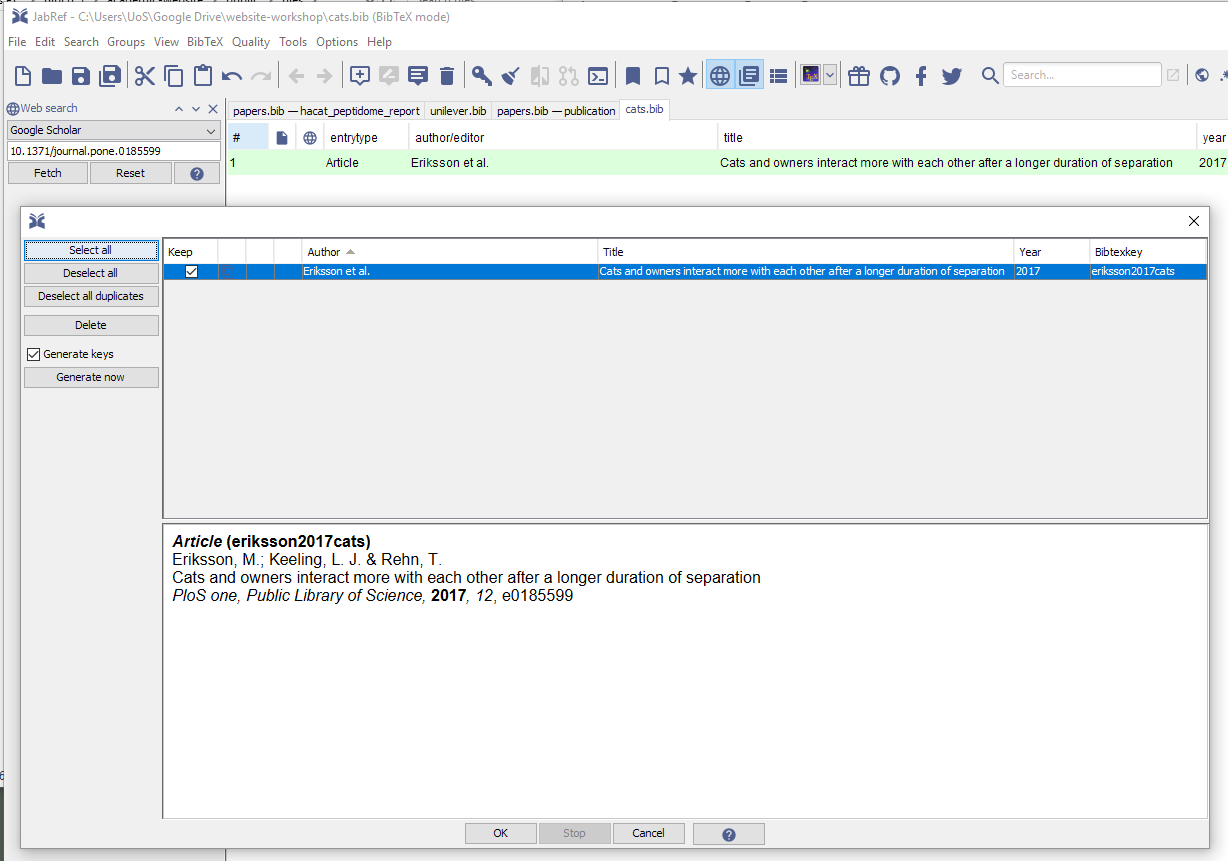
\includegraphics[width=1.2\linewidth]{img/jabref_websearch_2}

\begin{enumerate}
\def\labelenumi{\arabic{enumi}.}
\setcounter{enumi}{5}
\tightlist
\item
  Now we save the bibtex library. Here it is \texttt{cats.bib}. It's
  just another text file so can be viewed in any text editor.
\end{enumerate}

\section{Converting Bibtex files}\label{converting-bibtex-files}

Converting to markdown requires some effort, fortunately
\href{https://lbusett.netlify.com/post/automatically-importing-publications-from-bibtex-to-a-hugo-academic-blog/}{Lorenzo
Buesetto} wrote a function that required a small hack to work with
JabRef.

I found the function still may output files that need a bit of cleaning
up, but generally it works really well.

We need the \texttt{tidyverse,\ RefManageR,\ anytime} packages
installed.

\begin{Shaded}
\begin{Highlighting}[]
\NormalTok{bibtex_2academic <-}\StringTok{ }\ControlFlowTok{function}\NormalTok{(bibfile,}
\NormalTok{                             outfold,}
                             \DataTypeTok{abstract =} \OtherTok{FALSE}\NormalTok{,}
                             \DataTypeTok{overwrite =} \OtherTok{FALSE}\NormalTok{) \{}
                             \KeywordTok{require}\NormalTok{(RefManageR)}
                             \KeywordTok{require}\NormalTok{(dplyr)}
                             \KeywordTok{require}\NormalTok{(stringr)}
                             \KeywordTok{require}\NormalTok{(anytime)}
                             
                             \CommentTok{# Import the bibtex file and convert to data.frame}
\NormalTok{                             mypubs   <-}
\StringTok{                             }\KeywordTok{ReadBib}\NormalTok{(bibfile, }\DataTypeTok{check =} \StringTok{"warn"}\NormalTok{, }
                                     \DataTypeTok{.Encoding =} \StringTok{"UTF-8"}\NormalTok{) }\OperatorTok
\StringTok{                             }\KeywordTok{as.data.frame}\NormalTok{()}
                             
                             \CommentTok{# assign "categories" to the different types of}
                             \CommentTok{# publications}
\NormalTok{                             mypubs   <-}\StringTok{ }\NormalTok{mypubs }\OperatorTok
\StringTok{                             }\NormalTok{dplyr}\OperatorTok{::}\KeywordTok{mutate}\NormalTok{(}
                             \DataTypeTok{pubtype =}\NormalTok{ dplyr}\OperatorTok{::}\KeywordTok{case_when}\NormalTok{(}
\NormalTok{                             bibtype }\OperatorTok{==}\StringTok{ "Article"} \OperatorTok{~}\StringTok{ "2"}\NormalTok{,}
\NormalTok{                             bibtype }\OperatorTok{==}\StringTok{ "Article in Press"} \OperatorTok{~}\StringTok{ "2"}\NormalTok{,}
\NormalTok{                             bibtype }\OperatorTok{==}\StringTok{ "InProceedings"} \OperatorTok{~}\StringTok{ "1"}\NormalTok{,}
\NormalTok{                             bibtype }\OperatorTok{==}\StringTok{ "Proceedings"} \OperatorTok{~}\StringTok{ "1"}\NormalTok{,}
\NormalTok{                             bibtype }\OperatorTok{==}\StringTok{ "Conference"} \OperatorTok{~}\StringTok{ "1"}\NormalTok{,}
\NormalTok{                             bibtype }\OperatorTok{==}\StringTok{ "Conference Paper"} \OperatorTok{~}\StringTok{ "1"}\NormalTok{,}
\NormalTok{                             bibtype }\OperatorTok{==}\StringTok{ "MastersThesis"} \OperatorTok{~}\StringTok{ "3"}\NormalTok{,}
\NormalTok{                             bibtype }\OperatorTok{==}\StringTok{ "PhdThesis"} \OperatorTok{~}\StringTok{ "3"}\NormalTok{,}
\NormalTok{                             bibtype }\OperatorTok{==}\StringTok{ "Manual"} \OperatorTok{~}\StringTok{ "4"}\NormalTok{,}
\NormalTok{                             bibtype }\OperatorTok{==}\StringTok{ "TechReport"} \OperatorTok{~}\StringTok{ "4"}\NormalTok{,}
\NormalTok{                             bibtype }\OperatorTok{==}\StringTok{ "Book"} \OperatorTok{~}\StringTok{ "5"}\NormalTok{,}
\NormalTok{                             bibtype }\OperatorTok{==}\StringTok{ "InCollection"} \OperatorTok{~}\StringTok{ "6"}\NormalTok{,}
\NormalTok{                             bibtype }\OperatorTok{==}\StringTok{ "InBook"} \OperatorTok{~}\StringTok{ "6"}\NormalTok{,}
\NormalTok{                             bibtype }\OperatorTok{==}\StringTok{ "Misc"} \OperatorTok{~}\StringTok{ "0"}\NormalTok{,}
                             \OtherTok{TRUE} \OperatorTok{~}\StringTok{ "0"}
\NormalTok{                             )}
\NormalTok{                             )}
                             
                             \CommentTok{# create a function which populates the md template }
                             \CommentTok{# based on the info}
                             \CommentTok{# about a publication}
\NormalTok{                             create_md <-}\StringTok{ }\ControlFlowTok{function}\NormalTok{(x) \{}
                             \CommentTok{# define a date and create filename by appending date }
                             \CommentTok{# and start of title}
                             \ControlFlowTok{if}\NormalTok{ (}\OperatorTok{!}\KeywordTok{is.na}\NormalTok{(x[[}\StringTok{"year"}\NormalTok{]])) \{}
\NormalTok{                             x[[}\StringTok{"date"}\NormalTok{]] <-}\StringTok{ }\KeywordTok{paste0}\NormalTok{(x[[}\StringTok{"year"}\NormalTok{]], }\StringTok{"-01-01"}\NormalTok{)}
\NormalTok{                             \} }\ControlFlowTok{else}\NormalTok{ \{}
\NormalTok{                             x[[}\StringTok{"date"}\NormalTok{]] <-}\StringTok{ "2999-01-01"}
\NormalTok{                             \}}
                             
\NormalTok{                             filename <-}\StringTok{ }\KeywordTok{paste}\NormalTok{(}
\NormalTok{                             x[[}\StringTok{"date"}\NormalTok{]],}
\NormalTok{                             x[[}\StringTok{"title"}\NormalTok{]] }\OperatorTok
\StringTok{                             }\KeywordTok{str_replace_all}\NormalTok{(}\KeywordTok{fixed}\NormalTok{(}\StringTok{" "}\NormalTok{), }\StringTok{"_"}\NormalTok{) }\OperatorTok
\StringTok{                             }\KeywordTok{str_remove_all}\NormalTok{(}\KeywordTok{fixed}\NormalTok{(}\StringTok{":"}\NormalTok{)) }\OperatorTok
\StringTok{                             }\KeywordTok{str_sub}\NormalTok{(}\DecValTok{1}\NormalTok{, }\DecValTok{20}\NormalTok{) }\OperatorTok
\StringTok{                             }\KeywordTok{paste0}\NormalTok{(}\StringTok{".md"}\NormalTok{),}
                             \DataTypeTok{sep =} \StringTok{"_"}
\NormalTok{                             )}
                             \CommentTok{# start writing}
                             \ControlFlowTok{if}\NormalTok{ (}\OperatorTok{!}\KeywordTok{file.exists}\NormalTok{(}\KeywordTok{file.path}\NormalTok{(outfold, filename)) }\OperatorTok{|}
\StringTok{                             }\NormalTok{overwrite) \{}
\NormalTok{                             fileConn <-}\StringTok{ }\KeywordTok{file.path}\NormalTok{(outfold, filename)}
                             \KeywordTok{write}\NormalTok{(}\StringTok{"+++"}\NormalTok{, fileConn)}
                             
                             \CommentTok{# Title and date}
                             \KeywordTok{write}\NormalTok{(}\KeywordTok{paste0}\NormalTok{(}\StringTok{"title = }\CharTok{\textbackslash{}"}\StringTok{"}\NormalTok{, x[[}\StringTok{"title"}\NormalTok{]], }\StringTok{"}\CharTok{\textbackslash{}"}\StringTok{"}\NormalTok{),}
\NormalTok{                             fileConn,}
                             \DataTypeTok{append =}\NormalTok{ T)}
                             \KeywordTok{write}\NormalTok{(}\KeywordTok{paste0}\NormalTok{(}\StringTok{"date = }\CharTok{\textbackslash{}"}\StringTok{"}\NormalTok{, }\KeywordTok{anydate}\NormalTok{(x[[}\StringTok{"date"}\NormalTok{]]), }\StringTok{"}\CharTok{\textbackslash{}"}\StringTok{"}\NormalTok{),}
\NormalTok{                             fileConn,}
                             \DataTypeTok{append =}\NormalTok{ T)}
                             
                             \CommentTok{# Authors. Comma separated list, e.g. `["Bob Smith", }
                             \CommentTok{# "David Jones"]`.}
\NormalTok{                             auth_hugo <-}
\StringTok{                             }\KeywordTok{str_replace_all}\NormalTok{(x[}\StringTok{"author"}\NormalTok{], }\StringTok{" and "}\NormalTok{, }\StringTok{"}\CharTok{\textbackslash{}"}\StringTok{, }\CharTok{\textbackslash{}"}\StringTok{"}\NormalTok{)}
\NormalTok{                             auth_hugo <-}
\StringTok{                             }\NormalTok{stringi}\OperatorTok{::}\KeywordTok{stri_trans_general}\NormalTok{(auth_hugo, }\StringTok{"latin-ascii"}\NormalTok{)}
                             \KeywordTok{write}\NormalTok{(}\KeywordTok{paste0}\NormalTok{(}\StringTok{"authors = [}\CharTok{\textbackslash{}"}\StringTok{"}\NormalTok{, auth_hugo, }\StringTok{"}\CharTok{\textbackslash{}"}\StringTok{]"}\NormalTok{),}
\NormalTok{                             fileConn,}
                             \DataTypeTok{append =}\NormalTok{ T)}
                             
                             \CommentTok{# Publication type. Legend:}
                             \CommentTok{# 0 = Uncategorized, 1 = Conference paper, }
                             \CommentTok{# 2 = Journal article}
                             \CommentTok{# 3 = Manuscript, 4 = Report, 5 = Book,  6 = Book}
                             \CommentTok{# section}
                             \KeywordTok{write}\NormalTok{(}\KeywordTok{paste0}\NormalTok{(}\StringTok{"publication_types = [}\CharTok{\textbackslash{}"}\StringTok{"}\NormalTok{, x[[}\StringTok{"pubtype"}\NormalTok{]],}
                                          \StringTok{"}\CharTok{\textbackslash{}"}\StringTok{]"}\NormalTok{),}
\NormalTok{                             fileConn,}
                             \DataTypeTok{append =}\NormalTok{ T)}
                             
                             \CommentTok{# Publication details: journal, volume, issue, }
                             \CommentTok{# page numbers and doi link}
\NormalTok{                             publication <-}\StringTok{ }\NormalTok{x[[}\StringTok{"journal"}\NormalTok{]]}
                             \ControlFlowTok{if}\NormalTok{ (}\OperatorTok{!}\KeywordTok{is.na}\NormalTok{(x[[}\StringTok{"volume"}\NormalTok{]]))}
\NormalTok{                             publication <-}\StringTok{ }\KeywordTok{paste0}\NormalTok{(publication,}
                             \StringTok{", ("}\NormalTok{, x[[}\StringTok{"volume"}\NormalTok{]], }\StringTok{")"}\NormalTok{)}
                             \ControlFlowTok{if}\NormalTok{ (}\OperatorTok{!}\KeywordTok{is.na}\NormalTok{(x[[}\StringTok{"pages"}\NormalTok{]]))}
\NormalTok{                             publication <-}\StringTok{ }\KeywordTok{paste0}\NormalTok{(publication,}
                             \StringTok{", _pp. "}\NormalTok{, x[[}\StringTok{"pages"}\NormalTok{]], }\StringTok{"_"}\NormalTok{)}
                             \ControlFlowTok{if}\NormalTok{ (}\OperatorTok{!}\KeywordTok{is.na}\NormalTok{(x[[}\StringTok{"doi"}\NormalTok{]]))}
\NormalTok{                             publication <-}\StringTok{ }\KeywordTok{paste0}\NormalTok{(publication,}
                             \StringTok{", "}\NormalTok{,}
                             \KeywordTok{paste0}\NormalTok{(}\StringTok{"https://doi.org/"}\NormalTok{,}
\NormalTok{                             x[[}\StringTok{"doi"}\NormalTok{]]))}
                             
                             \KeywordTok{write}\NormalTok{(}\KeywordTok{paste0}\NormalTok{(}\StringTok{"publication = }\CharTok{\textbackslash{}"}\StringTok{"}\NormalTok{, publication, }\StringTok{"}\CharTok{\textbackslash{}"}\StringTok{"}\NormalTok{),}
\NormalTok{                             fileConn,}
                             \DataTypeTok{append =}\NormalTok{ T)}
                             \KeywordTok{write}\NormalTok{(}\KeywordTok{paste0}\NormalTok{(}\StringTok{"publication_short = }\CharTok{\textbackslash{}"}\StringTok{"}\NormalTok{,}
\NormalTok{                             publication,}
                             \StringTok{"}\CharTok{\textbackslash{}"}\StringTok{"}\NormalTok{),}
\NormalTok{                             fileConn,}
                             \DataTypeTok{append =}\NormalTok{ T)}
                             
                             \CommentTok{# Abstract and optional shortened version.}
                             \ControlFlowTok{if}\NormalTok{ (abstract) \{}
                             \KeywordTok{write}\NormalTok{(}\KeywordTok{paste0}\NormalTok{(}\StringTok{"abstract = }\CharTok{\textbackslash{}"}\StringTok{"}\NormalTok{, x[[}\StringTok{"abstract"}\NormalTok{]], }\StringTok{"}\CharTok{\textbackslash{}"}\StringTok{"}\NormalTok{),}
\NormalTok{                             fileConn,}
                             \DataTypeTok{append =}\NormalTok{ T)}
\NormalTok{                             \} }\ControlFlowTok{else}\NormalTok{ \{}
                             \KeywordTok{write}\NormalTok{(}\StringTok{"abstract = }\CharTok{\textbackslash{}"\textbackslash{}"}\StringTok{"}\NormalTok{,}
\NormalTok{                             fileConn,}
                             \DataTypeTok{append =}\NormalTok{ T)}
\NormalTok{                             \}}
                             \KeywordTok{write}\NormalTok{(}\KeywordTok{paste0}\NormalTok{(}\StringTok{"abstract_short = }\CharTok{\textbackslash{}"}\StringTok{"}\NormalTok{, }\StringTok{"}\CharTok{\textbackslash{}"}\StringTok{"}\NormalTok{),}
\NormalTok{                             fileConn,}
                             \DataTypeTok{append =}\NormalTok{ T)}
                             
                             \CommentTok{# other possible fields are kept empty. They can be}
                             \CommentTok{# customized later by}
                             \CommentTok{# editing the created md}
                             
                             \KeywordTok{write}\NormalTok{(}\StringTok{"image_preview = }\CharTok{\textbackslash{}"\textbackslash{}"}\StringTok{"}\NormalTok{,}
\NormalTok{                             fileConn,}
                             \DataTypeTok{append =}\NormalTok{ T)}
                             \KeywordTok{write}\NormalTok{(}\StringTok{"selected = false"}\NormalTok{, fileConn, }\DataTypeTok{append =}\NormalTok{ T)}
                             \KeywordTok{write}\NormalTok{(}\StringTok{"projects = []"}\NormalTok{, fileConn, }\DataTypeTok{append =}\NormalTok{ T)}
                             \KeywordTok{write}\NormalTok{(}\StringTok{"tags = []"}\NormalTok{, fileConn, }\DataTypeTok{append =}\NormalTok{ T)}
                             \CommentTok{#links}
                             \KeywordTok{write}\NormalTok{(}\StringTok{"url_pdf = }\CharTok{\textbackslash{}"\textbackslash{}"}\StringTok{"}\NormalTok{, fileConn, }\DataTypeTok{append =}\NormalTok{ T)}
                             \KeywordTok{write}\NormalTok{(}\StringTok{"url_preprint = }\CharTok{\textbackslash{}"\textbackslash{}"}\StringTok{"}\NormalTok{,}
\NormalTok{                             fileConn,}
                             \DataTypeTok{append =}\NormalTok{ T)}
                             \KeywordTok{write}\NormalTok{(}\StringTok{"url_code = }\CharTok{\textbackslash{}"\textbackslash{}"}\StringTok{"}\NormalTok{, fileConn, }\DataTypeTok{append =}\NormalTok{ T)}
                             \KeywordTok{write}\NormalTok{(}\StringTok{"url_dataset = }\CharTok{\textbackslash{}"\textbackslash{}"}\StringTok{"}\NormalTok{,}
\NormalTok{                             fileConn,}
                             \DataTypeTok{append =}\NormalTok{ T)}
                             \KeywordTok{write}\NormalTok{(}\StringTok{"url_project = }\CharTok{\textbackslash{}"\textbackslash{}"}\StringTok{"}\NormalTok{,}
\NormalTok{                             fileConn,}
                             \DataTypeTok{append =}\NormalTok{ T)}
                             \KeywordTok{write}\NormalTok{(}\StringTok{"url_slides = }\CharTok{\textbackslash{}"\textbackslash{}"}\StringTok{"}\NormalTok{, fileConn, }\DataTypeTok{append =}\NormalTok{ T)}
                             \KeywordTok{write}\NormalTok{(}\StringTok{"url_video = }\CharTok{\textbackslash{}"\textbackslash{}"}\StringTok{"}\NormalTok{, fileConn, }\DataTypeTok{append =}\NormalTok{ T)}
                             \KeywordTok{write}\NormalTok{(}\StringTok{"url_poster = }\CharTok{\textbackslash{}"\textbackslash{}"}\StringTok{"}\NormalTok{, fileConn, }\DataTypeTok{append =}\NormalTok{ T)}
                             \KeywordTok{write}\NormalTok{(}\StringTok{"url_source = }\CharTok{\textbackslash{}"\textbackslash{}"}\StringTok{"}\NormalTok{, fileConn, }\DataTypeTok{append =}\NormalTok{ T)}
                             \CommentTok{#other stuff}
                             \KeywordTok{write}\NormalTok{(}\StringTok{"math = true"}\NormalTok{, fileConn, }\DataTypeTok{append =}\NormalTok{ T)}
                             \KeywordTok{write}\NormalTok{(}\StringTok{"highlight = true"}\NormalTok{, fileConn, }\DataTypeTok{append =}\NormalTok{ T)}
                             \CommentTok{# Featured image}
                             \KeywordTok{write}\NormalTok{(}\StringTok{"[header]"}\NormalTok{, fileConn, }\DataTypeTok{append =}\NormalTok{ T)}
                             \KeywordTok{write}\NormalTok{(}\StringTok{"image = }\CharTok{\textbackslash{}"\textbackslash{}"}\StringTok{"}\NormalTok{, fileConn, }\DataTypeTok{append =}\NormalTok{ T)}
                             \KeywordTok{write}\NormalTok{(}\StringTok{"caption = }\CharTok{\textbackslash{}"\textbackslash{}"}\StringTok{"}\NormalTok{, fileConn, }\DataTypeTok{append =}\NormalTok{ T)}
                             
                             \KeywordTok{write}\NormalTok{(}\StringTok{"+++"}\NormalTok{, fileConn, }\DataTypeTok{append =}\NormalTok{ T)}
\NormalTok{                             \}}
\NormalTok{                             \}}
                             \CommentTok{# apply the "create_md" function over the }
                             \CommentTok{# publications list to generate}
                             \CommentTok{# the different "md" files.}
                             
                             \KeywordTok{apply}\NormalTok{(}
\NormalTok{                             mypubs,}
                             \DataTypeTok{FUN =} \ControlFlowTok{function}\NormalTok{(x)}
                             \KeywordTok{create_md}\NormalTok{(x),}
                             \DataTypeTok{MARGIN =} \DecValTok{1}
\NormalTok{                             )}
\NormalTok{                             \}}
\end{Highlighting}
\end{Shaded}

To use this function, save it as \texttt{bibtex\_2academic.R} and then
load the fcuntion into your R environment using
\texttt{source("bibtex\_2academic.R")}.

Then assuming you have a JabRef outputted Bixbtex file, here
\texttt{cats.bib} we need to assign variables for the bibtex file and
the output location, which in this case will be
\texttt{content/publication}. Then we use these variables as arguement
to the conversion function:

\begin{Shaded}
\begin{Highlighting}[]
\CommentTok{# Bibtex file in my directory}
\NormalTok{my_bibfile <-}\StringTok{ "cats.bib"}
\CommentTok{# Where I want the markdown output to go}
\NormalTok{outfold <-}\StringTok{ "content/publication"}
\CommentTok{# Use the conversion function}
\NormalTok{bibtex_2academic <-}\StringTok{ }\ControlFlowTok{function}\NormalTok{(my_bibfile,}
\NormalTok{                             outfold,}
                             \DataTypeTok{abstract =} \OtherTok{FALSE}\NormalTok{,}
                             \DataTypeTok{overwrite =} \OtherTok{FALSE}
\NormalTok{                             )}
\end{Highlighting}
\end{Shaded}

All being well, we should now have a markdown file for each publication
(we only had one in this example) in the \texttt{content/publication}.
It may need some manual tweaking if the format on the webpage isn't
quite right.

We can remove the example files that came with the template.

Bibi should now have her website configured and what's left is to
re-deploy the completed version which should look like this:


\includegraphics[width=1.2\linewidth]{img/bibi-final-site}

\chapter{Automating deployment with
GitHub}\label{automating-deployment-with-github}

In \protect\hyperlink{deployment}{Chapter 2} we used drag and drop of
the public folder, but if you are familiar with version control (and if
you aren't it's definitely worth learning), then you can automate
deployment using \href{https://github.com}{GitHub}.

The details are in the
\href{https://bookdown.org/yihui/blogdown/netlify.html}{blogdown book},
but essentially you can link netlify to your GitHub account and deploy
to netlify from there. This means that anytime you update your site in
Rstudio, you can push your files to GitHub and your site will be
deployed automatically.

Basically, this means you are tracking your changes and deploying in one
step, which is both quicker and means it's easy to revert should you
need to.

\bibliography{refs.bib,cats.bib,packages.bib}


\end{document}
